%% LyX 2.1.4 created this file.  For more info, see http://www.lyx.org/.
%% Do not edit unless you really know what you are doing.
\documentclass[english]{article}
\usepackage[T1]{fontenc}
\usepackage[latin9]{inputenc}
\usepackage{geometry}
\geometry{verbose,tmargin=2cm,bmargin=3cm,lmargin=1.5cm,rmargin=1.5cm}
\usepackage{float}
\usepackage{mathtools}
\usepackage{amsmath}
\usepackage{amssymb}
\usepackage{graphicx}
\usepackage{tablefootnote}
\usepackage{float}

\makeatletter

%%%%%%%%%%%%%%%%%%%%%%%%%%%%%% LyX specific LaTeX commands.
%% Because html converters don't know tabularnewline
\providecommand{\tabularnewline}{\\}
\floatstyle{ruled}
\newfloat{algorithm}{tbp}{loa}
\providecommand{\algorithmname}{Algorithm}
\floatname{algorithm}{\protect\algorithmname}

%%%%%%%%%%%%%%%%%%%%%%%%%%%%%% User specified LaTeX commands.
\usepackage{tikz}
\usepackage{babel}
\renewcommand{\labelitemi}{$\diamond$}
\newcommand{\T}{\rule{0pt}{2.6ex}}       % Top strut
\newcommand{\B}{\rule[-1.2ex]{0pt}{0pt}} % Bottom strut
\renewcommand{\vec}[1]{\boldsymbol{\mathbf{#1}}} % Vectors
\newcommand{\mat}[1]{\boldsymbol{\mathbf{#1}}} % Matrices
\usepackage{algorithm,algpseudocode}

\makeatother

\usepackage{babel}
\begin{document}

\title{COMP8620: MC-AIXI-CTW\\
Group 3}


\author{Jarryd Martin, Ryk Budzynski, John Aslanides,\\
Yadunandan Sannappa, Nrupendra Rao, \& Cheng Yu}


\date{October 2015}

\maketitle
\begin{abstract}
We outline an implementation of Veness et al.'s Monte Carlo AIXI approximation\cite{veness-11}
(MC-AIXI-CTW), and report our simulation results on a number of toy domains.
\end{abstract}

\tableofcontents{}

\section{Introduction}

Recall that the AIXI agent is defined by its actions, which for each
cycle $k$ are given by 
\[
a_{k}^{\text{AIXI}}=\arg\max_{a_{k}}\sum_{o_{k}r_{k}}\cdots\max_{a_{m}}\sum_{o_{m}r_{m}}\left[r_{k}+\dots+r_{m}\right]\xi\left(o_{1}r_{1}\dots o_{m}r_{m}|a_{1}\dots a_{m}\right),
\]

where the $o_{n}$ and $r_{n}$ are the observation and reward provided
by the environment at cycle $n$, and $\xi$ is a Bayesian mixture
model for the environment. 

Following Veness et al., we approximate $a_{k}^{\text{AIXI}}$ using
Monte Carlo tree search (upper confidence bound) to approximate the
expectimax, and we compute a mixture over variable-order Markov models
using the context-tree weighting algorithm. 

We present a lightweight C++ implementation of MC-AIXI-CTW, along
with implementations of a number of simple games: $\textsc{Pacman},\ $
$\textsc{Tic-Tac-Toe}$, $\textsc{Biased Rock-Paper-Scissor}$, $\textsc{Extended-Tiger}$,
and $\textsc{Cheesemaze}$.

\section{MC-AIXI-CTW Implementation}

In this section we outline the implementation of the agent, and its interface with its environments. 

\subsection{Agent-environment interaction loop}

For each agent-environment interaction cycle, we run the following
for each experiment (see Algorithm \ref{mainlopp}):

\begin{algorithm}[h]
\begin{algorithmic}[1]
\renewcommand{\algorithmicrequire}{\textbf{Inputs:}}
\renewcommand{\algorithmicensure}{\textbf{Outputs:}}
\While{$cycle < max\_cycles$}
\While{environment is not finished}
\State{generate $(o,r)$ from environment}
\State{update agent model with $(o,r)$}
\If{explore}
\State{$a \leftarrow randomAction()$}
\Else
\State{$a \leftarrow MCTS()$}
\Comment{Monte Carlo Tree Search}
\EndIf
\State{perform action $a$}
\State{update agent history with $a$}
\State{$cycle++$}
\EndWhile
\State{reset environment}
\EndWhile
\end{algorithmic}

\caption{Main loop.}
\label{mainloop}

\end{algorithm}

Essentially, the agent plays a turn-based game with its environment. The input tape of the agent is the output tape of the environment, and visa versa. Each cycle then adds an $(\text{observation},\text{reward},\text{action})$ triplet to the agent's history. The agent chooses actions according to its policy, and updates its internal model with observations from the environment. The agent's behavior is broken into three main modules: $\tt{search.cpp}$, $\tt{agent.cpp}$, and $\tt{predict.cpp}$.

The $MCTS$ algorithm can be found in its entirety in ${\tt search.cpp}$. Model updates and queries are handled by public methods in ${\tt agent.cpp}$, which interfaces with the (private) context tree
defined in ${\tt predict.cpp}$. Below, we detail the design and implementation of each of these modules.

\subsection{Monte Carlo Tree Search (MCTS) Algorithm}

The MCTS module comprises the planning part of the agent; it makes up the `sequential decision theory' section of the AIXI model. At each agent-environment interaction cycle, we wish to choose the action which maximises our total expected future reward, under the current policy and our best model of the environment. MCTS is a standard algorithm for collecting statistics and estimating the value $\hat{V}$ of each history. The MC-UTS (upper confidence bound tree search) algorithm is an adaptation of MCTS which adapts the UCB algorithm from bandit to manage exploration of the search space.

\subsubsection{High level description}

Note that pseudocode for the MC-UTS algorithm is presented in Veness et al., in Algorithms 1-4, so  we won't repeat their exposition here. Instead, we will outline the algorithm conceptually, and address some of the concerns in its implementation.

Since the environment is only partially observable, we have no explicit
notion of state; instead, we only have a history of actions and percepts
$h=\left(a_{1}o_{1}r_{1}\dots a_{n}o_{n}r_{n}\right)$. For the purposes
of choosing the optimal action, we treat each possible (hypothetical)
history as a node in the search tree, with the root being the tip
of the current (realised) history. \\

The search tree is comprised of alternating layers of decision nodes and
chance nodes with the root being a decision node. Decision nodes correspond to the agent's turn, and chance nodes correspond to the environmnet's turn. The maximum branching
possible from decision nodes is the number of available actions in the given
environment while the maximum branching possible from chance nodes is equal
to the number of possible observations times the number of possible rewards.
We do however restrict branching in general to $100$ to avoid memory issues. If we have a branching factor exceeding this, we sample uniformly from the $100$ existing nodes.
This number is configurable in ${\tt search.cpp}$. \\

Each node is implicitly labelled by its history as chance nodes record the
hypothetical action taken while decision nodes record the hypothetical
observation and reward from the environment.
The expected value of each node in the search tree is equal to the
expected total (non-discounted) reward that would be accumulated from
that node, where the expectation is under the agent's current policy
and the agent's current model for the behavior of the environment. \\

Thus, for each node we keep a value estimate $\hat{V}$, and a count
of the number of times $T$ that node has been visited in search.
This is used to determine how we explore the search space using the
UCB algorithm, which, for each decision node picks (assuming $T\left(ha\right)>0$
for all actions)
\[
a_{\text{UCB}}=\arg\max_{a\in\mathcal{A}}\left\{ \frac{1}{m\left(\beta-\alpha\right)}\hat{V}\left(ha\right)+C\sqrt{\frac{\log T\left(h\right)}{T\left(ha\right)}}\right\} ,
\]

where $\mathcal{A}$ is the set of all permissible actions, $m$ is
the search horizon, $\beta-\alpha$ is the difference between the
minimal and maximal instantaneous reward, and $C$ is a parameter
controlling the propensity of the agent to explore less frequently-seen
histories. \\

Note that the expectimax search generalises all environments, be they stochastic or even adversarial, since the actions of an opponent can be modelled as a distribution conditioned on the history of the game. In this sense, everything is modelled as a stochastic, partially observable game between the agent and its environment. In the following, search nodes corresponding to agent moves `decision nodes', and nodes corresponding to Nature's moves `chance nodes'. \\

\subsubsection{Class structure}

To represent our search nodes, we define a base ${\tt SearchNode}$
class, from which ChanceNode and DecisionNode inherit. ChanceNode
and DecisionNode each have a ${\tt sample}$ method defined on them;
each of these methods is mutually recursive. For a given node $n$,
we keep its children in a dictionary keyed on the action or (observation,reward)
used to generate each child.

\subsubsection{Other Considerations}

In addition to the psuedocode presented in Veness et al., we implemented a solution
to allow us to decide on a per cycle basis whether or not to build a search tree from
scratch. In addition, we constructed routines which given an action taken by the
agent and an observation/reward received from the environment, would prune the search
tree accordingly. \\

The pruning of the search tree removes all subtrees begining with the chance nodes
directly below the root which correspond to the actions not taken by the agent and
as such are impossible future paths. Additionally, all subtrees begining with descision
nodes below the chance node (corresponding to the action taken) that do not match the
observation/reward received from the environment are pruned. As cycles progress
throughout an experiment, this represents a significant reduction in memory consumption. \\

Our final solution however did not implement pruning as our experimental results showed
unusual behaviour whereby the agent would appear to get stuck in certain game states.

\subsubsection{Efficiency/performance}

Between calls to ${\tt search}$, we retain much of the search tree,
pruning those nodes that are now inaccessible from the realised $(a,o,r)$
tuple that happened during the cycle. This allows us to avoid re-generating
similar search trees from similar positions. 


\subsection{Context Tree Weighting (CTW)}


\subsubsection{High level description of algorithm}


\subsubsection{Class structure}


\subsubsection{Code snippets}


\subsubsection{Efficiency/performance}


\section{Environments}
To test the effectiveness of the agent we developed 5 environment simulations which range in complexity from the relatively simple cheese maze to the much more complicated partially observable pacman game. The details of these environments with respect to their behaviour and implementation is discussed below. For technical convenience, our agent only handles non-negative rewards; for this reason, our environments are all implemented so as to have their minimum reward set to zero. In this way, our implementations differ from the environment specifications. For the purpose of plotting and analysis of the results, and for optimality calculations, we transform all rewards back to their original specified ranges, so as to facilitate comparison with Veness's benchmark results. Note that this additive reward transformation has no effect on the agent's behavior. \\

In all of the environments, the agent is given a static interface of possible actions it can perform. At any given game state, some (indeed many) of these actions may be illegal; in all games, illegal moves are punished with significant penalties.
\subsection{Cheese Maze}
Cheese Maze is an episodic, deterministic and partially observable game in which the agent is a mouse trying to find a piece of cheese in a two dimensional maze. The objective is to find the cheese in the fewest amount of moves, while avoiding running into walls. The episode ends when the agent finds the cheese. The actions available to the agent are:
\begin{center}
	\begin{tabular}{c | c}
		\textbf{Action} & \textbf{Code} \\
		\hline
		Move Up & 0 \\
		Move Right & 1 \\
		Move Left & 2 \\
		Move Down & 3 \\
		\hline
	\end{tabular}
\end{center}
The transformed rewards are given by
\begin{center}
	\begin{tabular}{c | c}
		\textbf{Action effect} & \textbf{Reward} \\ \hline
		Game start & 0 \\
		Agent bumps into wall & 0 \\
		Agent moves into free cell & 9 \\
		Agent finds cheese & 20 \\ \hline	
	\end{tabular}
\end{center}

\par
The configuration of the maze and initial states of the agent and the cheese are read from the configuration file, and are identical to those specified in Figure 5 in Veness et al. The maze is represented as the list of nodes as they would be visited by the depth first search algorithm. Mouse position and cheese position are simply the order of the node.\\
Each node of the maze is a structure which stores the percept corresponding to that node, along with an array of pointers to its neighbours. In case there is a wall on a particular side of the node then that pointer will be $\tt{NULL}$. \\

The optimal strategy in each episode of Cheese Maze is to perform the sequence of actions$\left(\tt{game\ start}\rightarrow \tt{right} \rightarrow \tt{down} \rightarrow \tt{down}\right)$. This yields a total reward of $8$ utils in $4$ cycles, giving an upper bound for the average reward per cycle of $2$. Average reward per cycle is the main metric with which we evaluate the agent's performance in this and all other environments.

\subsection{Extended Tiger}
Extended Tiger is an episodic stochastic game. This environment simulates two doors, behind one of which is a tiger, and the other a pot of gold. At the start of each episode the tiger is placed behind one of the doors with probability 0.5. The agent begins sitting down and it can perform the following actions:
\begin{center}
	\begin{tabular}{c | c}
		\textbf{Action} & \textbf{Code} \\ \hline
		Stand & 0 \\
		Listen & 1 \\
		Open left door & 2 \\
		Open right door & 3 \\ \hline	
	\end{tabular}
\end{center}
When the agent performs the $\tt{listen}$ action, the environment provides an observation that correctly identifies the location of the tiger with probability $p$ (parametrised in the configuration file). Otherwise, its observation is $0$:

\begin{center}
	\begin{tabular}{c | c}
		\textbf{Observation} & \textbf{Code} \\ \hline
		Agent does not perform listen action & 0 \\
		Tiger behind left door & 1 \\
		Tiger behind right door & 2 \\ \hline
	\end{tabular}
\end{center}
The agent is penalised for performing illegal moves, or for opening the door with the tiger. The episode ends when one of the doors is opened. The transformed rewards the agent receives in this environment are as follows:
\begin{center}
\begin{tabular}{c | c | c}
	\textbf{State} & \textbf{Action} & \textbf{Reward} \\ \hline
	sitting & stand & 99 \\
	sitting & open door & 90 \\
	sitting & listen & 99 \\
	standing & stand & 90 \\
	standing & open door with tiger & 0 \\
	standing & open door with gold & 30 \\
	standing & listen & 90 \\ \hline
\end{tabular}
\end{center}

Clearly the optimal strategy in Extended Tiger will be the sequence $\left(\tt{game\  start}\rightarrow\tt{listen}\ n\ times\rightarrow\tt{stand}\rightarrow\tt{open\ door}\right)$. To play optimally given a fixed false observation probability of $q=1-p$, it is sufficient to maximise our expected reward with respect to $n$ using this sequence of moves. Hence the expected average reward under the optimal policy can be approximated by
$$\mathbb{E}[r_{\text{avg}}] = \frac{30(1-q)^n - 100(1-(1-q)^n)-n-1}{n+3},$$
where the denominator is equal to the number of actions taken, and the numerator approximates the expected reward for opening the door signalled by the majority of observations. In case of ties, the agent would need to listen more to collect more data, but we omit this case for simplicity's sake, since we are interested in a loose upper bound with which to benchmark our performance. With a false observation probability of $q=0.15$, the optimal number of listen actions $n$ is $2$.

\subsection{Tic-Tac-Toe}
Tic-Tac-Toe is a fully observable adversarial game. In this environment, the agent plays numerous games of Tic-Tac-Toe against an opponent who plays randomly. The agent's moves are coded as 0-8 referring to the different positions of the board:
\begin{center}
	\begin{tabular}{c | c | c}
	0 & 1 & 2 \\ \hline
	3 & 4 & 5 \\ \hline
	6 & 7 & 8 \\	
	\end{tabular}
\end{center}
The agent's observations completely describe the current state of the board using 2 bits for each cell of the board:
\begin{center}
	\begin{tabular}{c | l}
	00 & Cell empty \\
	01 & Agent's cell \\
	02 & Opponent's cell \\
	\end{tabular}
\end{center}
The agent's (additively transformed) rewards are as follows:
\begin{center}
	\begin{tabular}{c | c}
	\textbf{Status} & \textbf{Reward} \\ \hline
	Illegal move & 0 \\
	Game is a draw & 4 \\
	Game won by agent & 5 \\
	Agent lost & 1 \\
	\end{tabular}
\end{center}

In our setup, the agent has the first move. Under the optimal policy, and against a random opponent, the agent should win within 3 or 4 moves with high probability. Assuming no illegal moves are taken, the optimal strategy yields an average reward per cycle (loosely) upper bounded by $\frac{2}{3}$, since a win corresponds to a reward of $2$. Taking into account draws and longer games, we expect the true tighest upper bound to be somewhere in the range $[0.5,\frac{2}{3}]$.

\subsection{Biased Rock-Paper-Scissors}
This is an adversarial, non-episodic game. The agent plays against an opponent who plays randomly, except when they win a round, in which case they will play the same move in the following round with probability $1$. We encode the actions of the agent and the environment as:
\begin{center}
	\begin{tabular}{c | c}
	Rock & 0 \\
	Paper & 1 \\
	Scissors & 2 \\
	\end{tabular}
\end{center}
The agent receives a reward of 1 for a win, 0 for a draw and -1 for a loss. \\

In terms of an optimal agent strategy, an upper bound on reward per cycle for Biased Rock-Paper-Scissors is derived as follows. Let $X_t$ be a random variable representing the outcome of cycle $t$. Under an optimal strategy, the agent will win after the environment won in cycle $t-1$ as the environments action in cycle $t$ is predictable. Otherwise, the agent should play randomly. Now, the probability of the agent's winning at time $t$ is given by
\begin{align*}
P(X_t = \text{win})&= \sum_{X_{t-1}} P(X_t = \text{win}, X_{t-1})\\ 
 &= \sum_{X_{t-1}} P(X_t = \text{win}|X_{t-1})P(X_{t-1}),
\end{align*}
which corresponds to a 1\textsuperscript{st} order Markov chain with the following right stochastic transition matrix

\begin{align}
\mat{P} = 
\begin{bmatrix}
\frac{1}{3} & \frac{1}{3} & \frac{1}{3} \\
1 & 0 & 0 \\
\frac{1}{3} & \frac{1}{3} & \frac{1}{3}
\end{bmatrix}
\end{align}

Therefore, we want a steady state distribution for $\mat{P}$, i.e. a solution to $\vec{\pi} = \mat{P}\vec{\pi}$. This is given by the eigenvector $\vec{\pi^{*}}$. The average reward at time $t$ is then
\begin{align*}
\mathbb{E}[r_{\text{avg}_t}] &= 1 \cdot P(X_t = \text{win}) + 0 \cdot P(X_t =\text{draw}) - 1 \cdot P(X_t = \text{lose})\\
 &= \vec{\pi^{*}_\text{win}} - \vec{\pi^{*}_\text{lose}} \\
 &= 0.25.
\end{align*}
\subsection{Partially Observable PacMan}
In contrast to standard PacMan, our implementation is partially observable, which makes it more difficult to play optimally, but more tractable computationally. The agent does not know the structure of the maze but only receives a 4 bit wall configuration of the node it is currently in. The agent also receives a 4 bit observation of the presence of any ghosts in its direct line of sight. The location of food pellets can change every episode as every free cell has a 50\% chance of having food in it. The agent receives a 3 bit observation indicating the presence of food within a Manhattan distance of 2, 3 or 4. It also receives a 4 bit string indicating food in its line of sight similar to the ghosts. The agent also knows whether it is under the effect of the power pill.\\
\begin{center}
	\begin{tabular}{c | c}
	\textbf{Action} & \textbf{Reward} \\ \hline
	Agent runs into a wall & -10 \\
	Agent caught by a ghost & -50 \\
	Agent moves into empty cell & -1 \\
	Agent eats a food pellet & 10 \\
	Agent collects all the food & 100 \\
	\end{tabular}
\end{center}
To obtain non-negative rewards for our agent, we transform this environment by adding $60$ to all reward percepts. This is because the agent can potentially be simultaneously caught by a ghost and run into a wall in the same cycle, resulting in the penalties being added.

The optimal strategy for PacMan is unknown, and so an upper bound on agent performance is unknown. Given that this is the most complex and demanding of our five environments, we can assume that without long training times and finely tuned agent learning parameters, learning in this game will be very difficult.

%%%%%%%%%%%%%%%%%%%%%%%%%%%%%%%
\section{Experiments}

\subsection{Experimental Setup}
Having implemented the MC-AIXI-CTW agent and five game environments, we proceed to run simulations. Our primary objective here is to test the agent against each of the environments, with the agent having no prior knowledge. During each experiment, we run the agent-environment loop for a large number of cycles (typically in the range of $[5\times 10^3,3\times 10^4]$), while maintaining the state of the agent's context tree model betwene cycles and episodes. \\

For each experiment, the agent's actions are controlled according to a training-evaluation schedule. During the training phase, the agent chooses a random action with probability $\epsilon$, and performs the normal Monte Carlo expectimax search otherwise. Over the course of the experiment, the exploration rate decays exponentially as $\epsilon_t = \epsilon_0 \gamma^t$. During evaluation cycles, the agent plans using the Monte Carlo tree search, and does no explicit exploration. We evaluate the agent's performance by plotting its average reward per cycle against \textit{evaluation} cycles. Typically, we alternate between $1000$ cycles of training, followed by $200$ cycles of evaluation, and repeat until the total allocated number of cycles is exhausted. 

In all of the following plots, we report the \textit{running} average reward per cycle $\bar{R}$, and the \textit{rolling} average reward per cycle $\tilde{R}$, which are defined as 

\begin{align*}
\bar{R}_t = \frac{1}{t}\sum_{i=1}^{t}{R_i}\\ 
\bar{R}^w_t = \frac{1}{w}\sum_{i=t-w}^{t}{R_i},
\end{align*}

for some sliding window $w>0$. For the last section of our experiments, we train MC-AIXI-CTW on Cheese Maze (CM), then train it on Rock-Paper-Scissor (RPS), before interfacing it again with Cheese Maze. The goal here is to see whether knowledge in CM is useful in RPS, and whether the agent retains any of its CM knowledge after a series of episodes training in RPS.

\subsection{Experiment Summary}
Here we summarise the parameters used in our experiments.\\

\begin{table}[H]
\begin{tabular}{|l|l|l|l|l|l|l|l|l|}
\hline 
 & $b$& $D$ & $n_\text{cycles}$& $t_\text{max}$ & $m$ & $\epsilon_0$  & $\gamma$ & $w_\text{UCB}$  \tabularnewline
\hline 
Cheesemaze & $11$ & $96$ & $10$ & $0.5$ & $8$ & $0.999$ & $0.99977$ & $1.4$ \tabularnewline
           & $11$ & $96$ & $10$ & $1.6$ & $6$ & $0.999$ & $0.99977$ & $1.4$ \tabularnewline
           & $11$ & $144$ & $2.5$ & $3$ & $8$ & $0.999$ & $0.99908$ & $1.4$ \tabularnewline
           & $11$ & $48$ & $10$ & $0.1$ & $4$ & $0.999$ & $0.99977$ & $1.4$ \tabularnewline
           & $11$ & $96$ & $10$ & $0.5$ & $8$ & $0.999$ & $0.99977$ & $1.4$ \tabularnewline
\hline
Biased Rock-Paper-Scissors & $6$ & $32$ & $10$ & $2.5$ & $4$ & $0.999$ & $0.9998$ & $1.4$ \tabularnewline
                           & $6$ & $48$ & $5$ & $5$ & $8$ & $0.999$ & $0.9995$ & $1.4$ \tabularnewline
                           & $6$ & $96$ & $4.5$ & $4$ & $4$ & $0.999$ & $0.9995$ & $1.4$ \tabularnewline
                           & $6$ & $96$ & $10$ & $0.5$ & $4$ & $0.999$ & $0.999$ & $1.4$ \tabularnewline
\hline
Extended Tiger & $13$ & $96$ & $16$ & $2.5$ & $6$ & $0.999$ & $0.9999$ & $1.4$ \tabularnewline
               & $13$ & $96$ & $2.5$ & $12$ & $4$ & $0.999$ & $0.99908$ & $1.4$ \tabularnewline
               & $13$ & $96$ & $25$ & $0.8$ & $4$ & $0.999$ & $0.999908$ & $1.4$ \tabularnewline
               & $13$ & $52$ & $5$ & $8$ & $4$ & $0.999$ & $0.99954$ & $1.4$ \tabularnewline
\hline
Tic-Tac-Toe    & $25$ & $96$ & $4.5$ & $4$ & $9$ & $0.9999$ & $0.99949$ & $1.4$ \tabularnewline
               & $25$ & $192$ & $5$ & $8$ & $9$ & $0.9999$ & $0.99954$ & $1.4$ \tabularnewline
               & $25$ & $256$ & $20$ & $8$ & $9$ & $0.9999$ & $0.99988$ & $1.4$ \tabularnewline
               & $25$ & $512$ & $25$ & $3$ & $9$ & $0.9999$ & $0.999908$ & $1.4$ \tabularnewline
               & $25$ & $512$ & $30$ & $2$ & $9$ & $0.9999$ & $0.99992$ & $1.4$ \tabularnewline
\hline
Pacman         & $26$ & $256$ & $10$ & $4$ & $8$ & $0.99$ & $0.999$ & $1.5$ \tabularnewline
               & $26$ & $512$ & $20$ & $2$ & $4$ & $0.9999$ & $0.99988$ & $1.4$ \tabularnewline
               & $26$ & $320$ & $10$ & $4$ & $8$ & $0.99$ & $0.999$ & $1.4$ \tabularnewline
               & $26$ & $256$ & $10$ & $1$ & $6$ & $0.9999$ & $0.99977$ & $1.4$ \tabularnewline
\hline 
\hline
\end{tabular}
\caption{MC-AIXI-CTW Experiments. Here, $b$ is the total bit length of an $(o,r,a)$ tuple, $D$ is the depth of the context tree, $n_\text{cycles}$ is the maximum number of global cycles allowed in the experiment, $t_\text{max}$ is the search time allowed per cycle, $m$ is the search horizon, $\epsilon_0$ is the initial exploration rate, $\gamma$ is the exploration decay rate, and $w_\text{UCB}$ is the UCB exploration bias parameter.}
\end{table}

\subsection{Cheesemaze}
Here we present the environmental setup and learning rate of our best results
training AIXI on the Cheesemaze environment. \\

Interpreting the results, we conclude that ... \\

\begin{table}[H]
\centering
\begin{tabular}{|l|l|l|l|l|l|l|l|}
\hline 
Bits & CT-depth & Cycles & Timeout & Horizon & Exp. Rate & Exp.-Decay & UCB-weight \tabularnewline
\hline 
$11$ & $96$ & $10$ & $0.5$ & $8$ & $0.999$ & $0.99977$ & $1.4$ \tabularnewline
\hline
\end{tabular}
\caption{Environment Setup}
\end{table}

\begin{figure}[h!]
\centering
\caption{Agent performance: Cheese Maze}
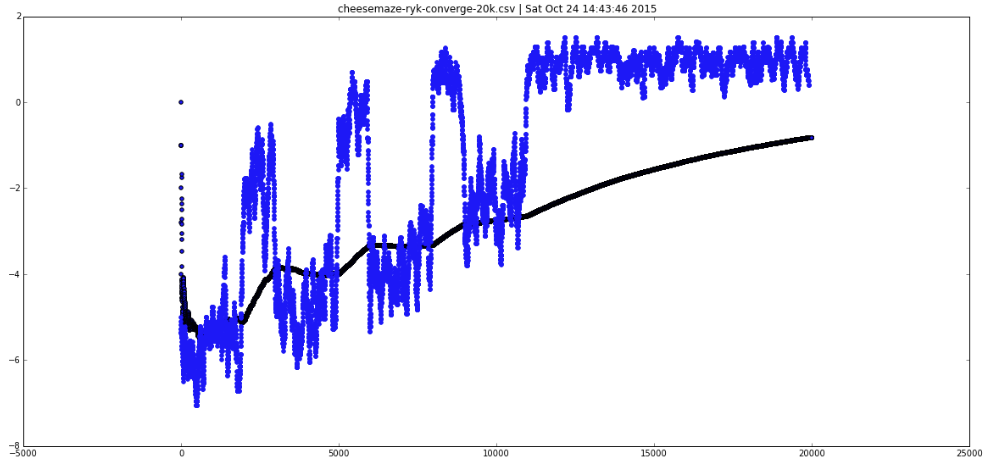
\includegraphics[scale=0.4]{cheesemaze_best} 
\end{figure}

\subsection{Extended Tiger}
Here we present the environmental setup and learning rate of our best results
training AIXI on the Extended Tiger environment. \\

Interpreting the results, we conclude that ... \\

\begin{table}[H]
\centering
\begin{tabular}{|l|l|l|l|l|l|l|l|}
\hline 
Bits & CT-depth & Cycles & Timeout & Horizon & Exp. Rate & Exp.-Decay & UCB-weight \tabularnewline
\hline 
$11$ & $96$ & $10$ & $0.5$ & $8$ & $0.999$ & $0.99977$ & $1.4$ \tabularnewline
\hline
\end{tabular}
\caption{Environment Setup}
\end{table}

\begin{figure}[H]
\centering
\caption{Agent performance: Extended Tiger}
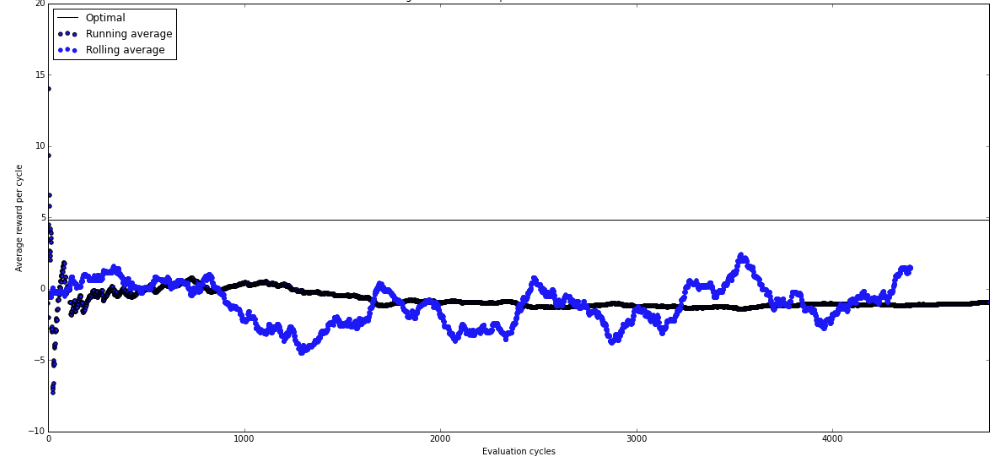
\includegraphics[scale=0.4]{tiger_best} 
\end{figure}

\subsection{Tic\-Tac\-Toe}
Here we present the environmental setup and learning rate of our best results
training AIXI on the Tic-Tac-Toe environment. \\

Interpreting the results, we conclude that ... \\

\begin{table}[H]
\centering
\begin{tabular}{|l|l|l|l|l|l|l|l|}
\hline 
Bits & CT-depth & Cycles & Timeout & Horizon & Exp. Rate & Exp.-Decay & UCB-weight \tabularnewline
\hline 
$11$ & $96$ & $10$ & $0.5$ & $8$ & $0.999$ & $0.99977$ & $1.4$ \tabularnewline
\hline
\end{tabular}
\caption{Environment Setup}
\end{table}

\begin{figure}[H]
\centering
\caption{Agent performance: Tic-Tac-Toe}
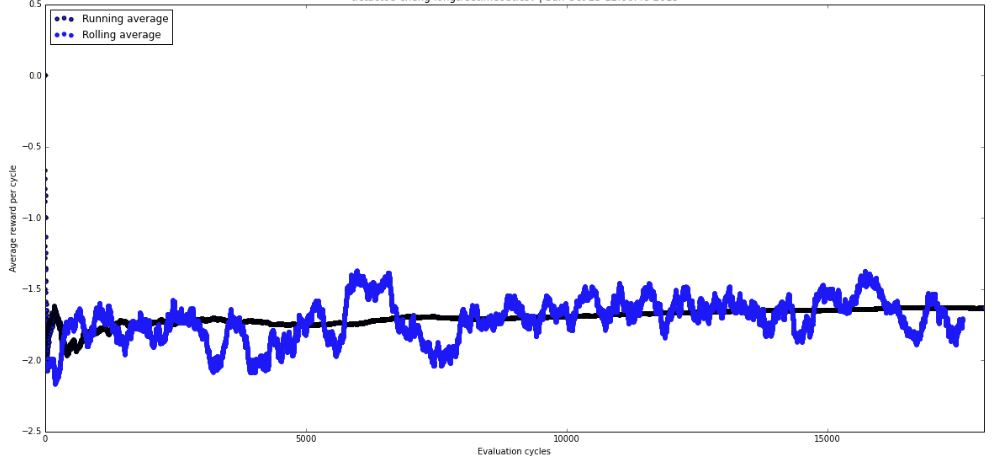
\includegraphics[scale=0.4]{tictactoe_best} 
\end{figure}

\subsection{Biased Rock-Paper-Scissors}
Here we present the environmental setup and learning rate of our best results
training AIXI on the Biased Rock-Paper-Scissors environment. \\

Interpreting the results, we conclude that ... \\

\begin{table}[H]
\centering
\begin{tabular}{|l|l|l|l|l|l|l|l|}
\hline 
Bits & CT-depth & Cycles & Timeout & Horizon & Exp. Rate & Exp.-Decay & UCB-weight \tabularnewline
\hline 
$11$ & $96$ & $10$ & $0.5$ & $8$ & $0.999$ & $0.99977$ & $1.4$ \tabularnewline
\hline
\end{tabular}
\caption{Environment Setup}
\end{table}

\begin{figure}[H]
\centering
\caption{Agent performance: Biased Rock-Paper-Scissors}
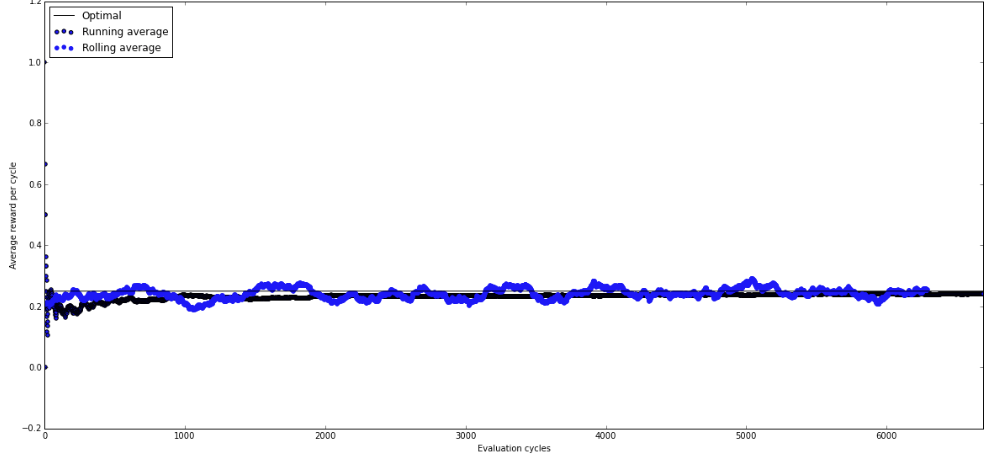
\includegraphics[scale=0.4]{rockpaper_best} 
\end{figure}

\subsection{Pacman}
Here we present the environmental setup and learning rate of our best results
training AIXI on the Pacman environment. \\

Interpreting the results, we conclude that ... \\

\begin{table}[H]
\centering
\begin{tabular}{|l|l|l|l|l|l|l|l|}
\hline 
Bits & CT-depth & Cycles & Timeout & Horizon & Exp. Rate & Exp.-Decay & UCB-weight \tabularnewline
\hline 
$11$ & $96$ & $10$ & $0.5$ & $8$ & $0.999$ & $0.99977$ & $1.4$ \tabularnewline
\hline
\end{tabular}
\caption{Environment Setup}
\end{table}

\begin{figure}[H]
\centering
\caption{Agent performance: PacMan}
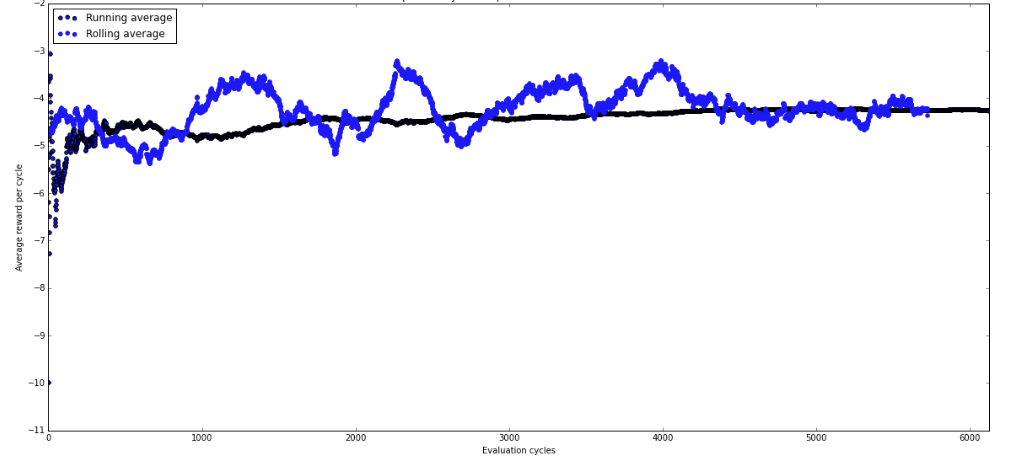
\includegraphics[scale=0.4]{pacman_best} 
\end{figure}

\subsection{Cross Domain Simulation Results}
\begin{itemize}
\item Cheesemaze and Biased Rock-Paper-Scissors
\item Cross domain simulation on more difficult environments... 
\end{itemize}
\begin{figure}[H]
\centering
\caption{Learning Rate}
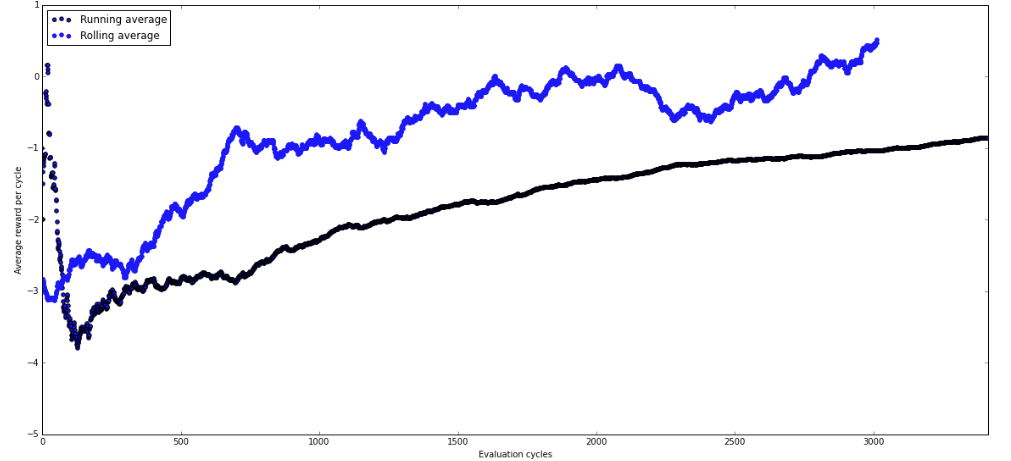
\includegraphics[scale=0.4]{cheeserock_1} 
\end{figure}

\begin{figure}[H]
\centering
\caption{Learning Rate}
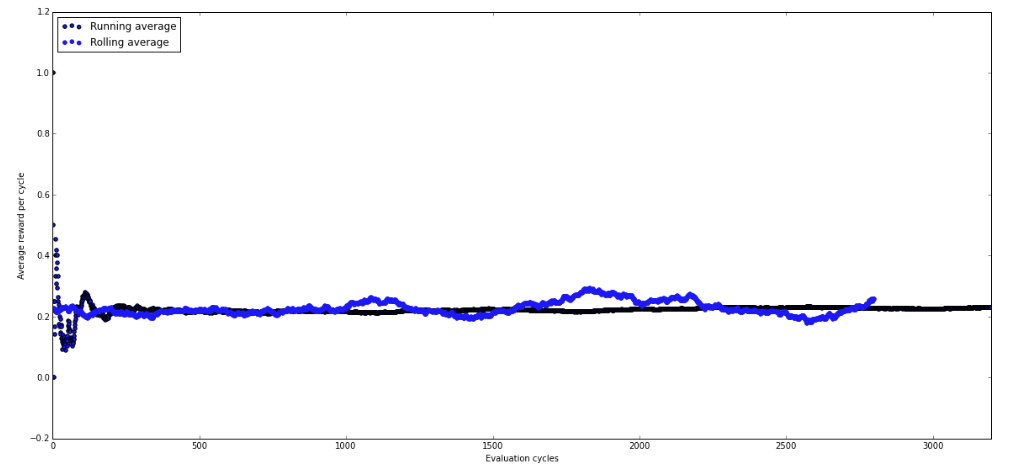
\includegraphics[scale=0.4]{cheeserock_2} 
\end{figure}

\begin{figure}[H]
\centering
\caption{Learning Rate}
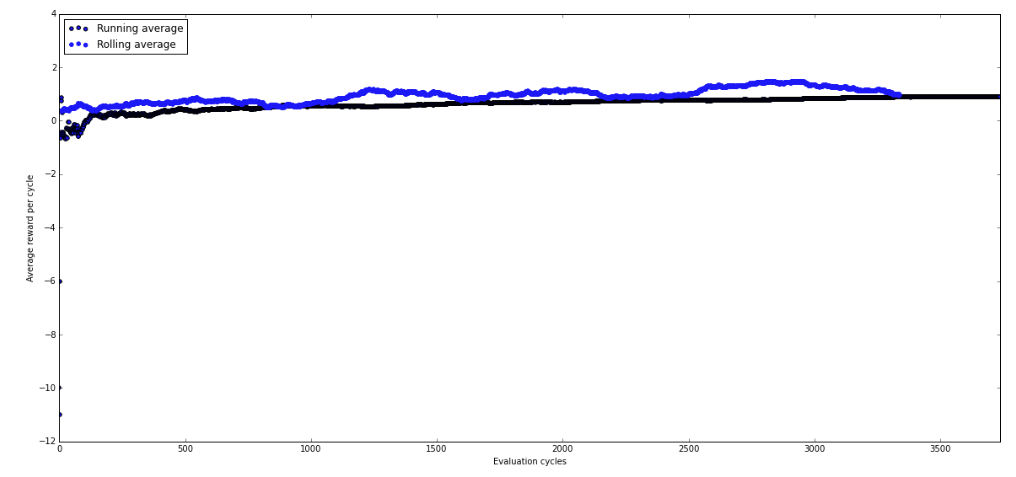
\includegraphics[scale=0.4]{cheeserock_3} 
\end{figure}

\section{Conclusion}



\section*{Appendix}

\appendix

\section*{User Manual}

To build from source on linux, run ${\tt g++\ -std=c++0x *.cpp\ -o\ aixi}$ \textbf{TODO
check}

To run, invoke ${\tt ./aixi\ \$ENVNAME.conf}$. 


\section{Files}

The report archive should contain the following: 
\begin{verbatim}

MC-AIXI-CTW-Grp3.zip
    \report
        report.pdf // this report
        report.tex
        cheesemaze_best.png // results plots
        tiger_best.png
        rockpaper_best.png
        tictactoe_best.png
        pacman_best.png
    \src
        main.hpp
        main.cpp
        environment.hpp
        environment.cpp
        agent.hpp
        agent.cpp
        search.hpp
        search.cpp
        predict.hpp
        predict.cpp
        util.hpp
        util.cpp
        README.md
        cheesemaze.conf // environment configuration files
        rockpaper.conf
        tictactoe.conf
        coinflip.conf
        tiger.conf
\end{verbatim}

\section{Plots}

\bibliographystyle{unsrt}
\bibliography{report}

\end{document}
